\chapter{Marco Teórico: conceptos teóricos}
\section{Comunicación}
La comunicación es un proceso dinámico, en el que participa una fuente o emisor que envía un mensaje a través de un canal o medio a un potencial receptor que, a su vez, puede convertirse también en emisor [16]. Cuando se transmite el mensaje de una forma clara y efectiva para el receptor sin generar dudas ni confusiones, se logra un comunicación efectiva [17].\\

Comunicar es el acto que permite establecer relaciones efectivas, compartir experiencias, experimentar emociones y sentimientos, así como hacer que los demás lo experimenten [18].

\subsection{Tipos de Comunicación}
Uno de los tipos de comunicación está basado en si se usan palabras o no, es decir, comunicación verbal o no verbal [20]:
\begin{itemize}
    \item Comunicación verbal: se emplean palabras, y se lleva a cabo a través del habla o de manera escrita.
\item Comunicación no verbal: se emplea el lenguaje corporal, gestos, signos no lingüísticos y sonidos que no forman palabras.
\end{itemize}
Otro de los tipos de comunicación son la formal y la informan, las cuales se describen a continuación:

\begin{itemize}

\item Formal: se utiliza un lenguaje especializado y estandarizado, sin errores ni coloquialismos, además de que se toman en cuenta las jerarquías sociales.
\item Informal: no se emplea lenguaje estandarizado, no se siguen protocolos jerárquicos y se emplean coloquialismos.
\end{itemize}
Un tercer tipo de clasificación es aquella que está basada en el tipo de acto comunicativo, la cual contiene los siguientes elementos [20]:
\begin{itemize}
\item Comunicación intrapersonal: conversaciones que un ser humano entabla consigo mismo.
\item Comunicación interpersonal: intercambio de ideas y pensamientos entre dos personas, la cuál debe ser directa e interactiva.
\item Comunicación grupal: intercambio de ideas y pensamientos entre un grupo de más de dos personas, las cuales se comunican con un propósito.
\item Comunicación masiva: comunicación dirigida a un gran número de personas, mediante un medio masivo de comunicación como lo puede ser las redes sociales, radio, televisión, entre otros.
\end{itemize}

\subsection{Elementos de la comunicación}
Dentro del proceso de comunicación hay una serie de elementos que hacen posible la transmisión de un mensaje. A continuación, se enlistan cada uno de ellos: 
\begin{itemize}
    
\item Emisor. El emisor es el individuo que inicia el intercambio de información al transmitir el mensaje [18]. Dicho mensaje debe ser codificado en un sistema de símbolos que deberá ser entendible para el receptor. 

\item Receptor. Individuo que recibe el mensaje enviado, el cual es interpretado con base en las experiencias, opiniones, contexto y situación del receptor [16]. El receptor también puede ser el emisor.

\item Código. Es el sistema de signos que es empleado tanto por el emisor como por el receptor para llevar a cabo el proceso de comunicación. Ese sistema debe ser conocido por ambos para facilitar la codificación y descodificación [20].

\item Mensaje. Es la información que el emisor transmite al receptor por medio del código [19].

\item Canal. El canal es el medio en el que los mensajes del emisor se transmiten hacia el receptor [16].

\item Contexto. Se refiere a la situación en la que se lleva a cabo el proceso de comunicación, la cual tiene influencia directa en el entendimiento e interpretación del mensaje [19].

\item Retroalimentación. Es la respuesta que el receptor emite tras haber recibido e interpretado un mensaje, convirtiéndose momentáneamente en emisor. Este elemento permite cerrar el ciclo comunicativo al brindar al emisor una señal clara sobre si su mensaje fue comprendido, aceptado o necesita ser aclarado o reformulado [20].

\item Ruido o interferencia. Dentro del proceso de comunicación puede haber factores externos que dificultan o impiden el entendimiento de los mensajes [20].
\end{itemize}

\begin{center}
    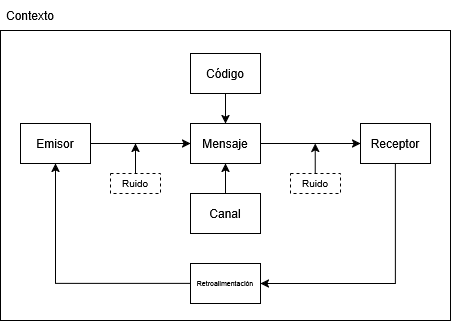
\includegraphics[width=0.8\textwidth]{Images/Cap 2/ProcesoComunicacion.png}
    \captionof{figure}{Proceso de comunicación, elaboración propia.} 
\end{center}

La comunicación es un proceso indispensable para la interacción humana ya que por medio de ella las personas pueden intercambiar ideas, pensamientos y emociones. No obstante, como se menciona en el concepto de ruido, en ocasiones hay elementos que impiden que la comunicación se lleve a cabo, como lo pueden ser las barreras de la comunicación.
\subsection{Barreras de la comunicación}
Las barreras de la comunicación son elementos que limitan o dificultan que las personas puedan comunicarse, a la par que se dificulta su proceso de comunicación [2]. Son todas las perturbaciones que sufre un mensaje, en cualquiera de los elementos que forman parte del proceso de comunicación.

Los principales tipos de barreras son:
\begin{enumerate}
    \item \textbf{Barreras físicas.} Son interferencias causadas por elementos del entorno o en el medio donde se lleva a cabo la comunicación [21].
    \item \textbf{Barreras psicológicas.} Son aquellas que surgen por emociones, prejuicios o estados mentales que afectan la interpretación del mensaje [21].
    \item \textbf{Barreras semánticas.} Surgen cuando hay confusión en el significado de las palabras, debido a una interpretación incorrecta del lenguaje. Generalmente ocurren cuando se habla en un idioma que el emisor o el receptor no entienden, o se emplean conceptos técnicos desconocidos [21].
    \item \textbf{Barreras administrativas.} Generalmente se presentan en entornos laborales y son causadas por falta de planeación, malentendidos, falta de claridad en los procesos de comunicación y distorsiones semánticas [21].
    \item \textbf{Barreras culturales.} Este tipo de barreras se presentan cuando hay diferencias en costumbres, valores, normas o expresiones entre culturas, que imposibilitan la comunicación [21].
    \item \textbf{Barreras interpersonales.} Hace referencia a las barreras en las que hay suposiciones incorrectas y diferentes percepciones [21].
    \item \textbf{Barreras tecnológicas.} Fallas y limitaciones que se presentan en medios tecnológicos empleados para la comunicación [21].
    \item \textbf{Barreras fisiológicas.} Impedimentos físicos o biológicos causados por deficiencias en los sentidos, enfermedades o condiciones médicas que afectan cualquiera de los sentidos de manera parcial o total, afectando la transmisión de información [21]. Por ejemplo, voz débil, pronunciación defectuosa, sordera, problemas del habla, problemas visuales, etc.
\end{enumerate}
Para efectos de este Trabajo Terminal se analizarán las barreras fisiológicas, concretamente las que son causadas por problemas de sordera. En el siguiente apartado se describen los términos correctos para referirse a las personas con capacidad de escucha y a las personas con discapacidad auditiva.\\

\section{Personas con discapacidad auditiva}
\subsection{Personas Oyentes}
Un oyente se define como aquella persona con la capacidad de escuchar sonidos que le permiten interpretar mensajes. El término procede del verbo oír, que refiere a la capacidad que posee un individuo para poder percibir sonidos [22].

\subsection{Personas con discapacidad auditiva (sordas)}
La discapacidad auditiva se define como la pérdida de la función del sistema auditivo, teniendo como consecuencia una discapacidad para poder oír, lo que dificulta el acceso al lenguaje oral [s1].\\ 

De acuerdo con la Federación Mundial de Sordos, existen aproximadamente 70 millones de personas sordas en todo el mundo, las cuales emplean más de 300 diferentes lenguas de señas [s2]. Las lenguas de señas varían entre países, presentando cambios principalmente en la estructura gramatical, sintaxis, vocabulario, signos, alfabeto y expresiones corporales [22].\\

Por otro lado, la Secretaría de Salud menciona que en México hay aproximadamente 2.3 millones de personas con discapacidad auditiva, de las cuales más del 50\% son mayores de 60 años, 34\% tienen entre 30 y 59 años, y el 2\% son niñas y niños [3].\\

Las principales causas de problemas de audición son antecedentes familiares de sordera heredados, edad avanzada, enfermedades infecciosas, exposición continua a sonidos intensos, entre otras [3].\\

Las personas sordas enfrentan consecuencias en ámbitos académicos, laborales, sociales y emocionales, debido a que las situaciones de aislamiento, deficiencia en la comunicación y dificultades del día a día repercuten negativamente para integrarse en grupos y para socializar [s21]. \\

\subsection{Tipos de Discapacidad Auditiva}
La discapacidad auditiva se clasifica en tres tipos según distintos criterios: según la parte del oído afectada, según el grado de pérdida auditiva y según el momento en que se adquiere [s22]:\\
\newline\textbf{Según la parte del oído afectada}
\begin{itemize}
    \item \textbf{Hipoacusia conductiva.} Es producida por un impedimento en el trayecto de las ondas sonoras del oído externo y medio al oído interno, causado por tumores, perforación del tímpano, traumatismos o disfunciones del oído.  
    \item \textbf{Hipoacusia neurosensorial.} Se produce cuando el nervio auditivo o las células ciliadas son dañadas, ya sea por herencia, anormalidades al momento del nacimiento, exposición a ruidos fuertes, traumatismos, entre otras causas.  
    \item \textbf{Hipoacusia mixta.} Combinación de hipoacusia conductiva e hipoacusia neurosensorial, causadas por anormalidades al nacer, infecciones, tumores y lesiones en la cabeza.  
\end{itemize}

\begin{center}
    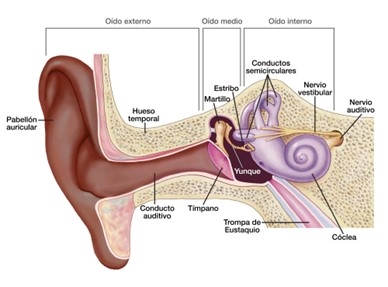
\includegraphics[width=0.8\textwidth]{Images/Cap 2/PartesOido.jpg}
    \captionof{figure}{Partes del oído humano, obtenido de [i2].} 
\end{center}

\textbf{Según el grado de pérdida}\\
El rango normal de audición oscila entre 0 y 20 decíbeles (dB). Tomando en consideración ese rango, se establece la siguiente clasificación de acuerdo con los dB que se hayan perdido:

\begin{itemize}
    \item \textbf{Leve:} 20-40 dB.  
    \item \textbf{Moderada:} 40-70 dB.  
    \item \textbf{Severa:} 70-90 dB.  
    \item \textbf{Profunda:} más de 90 dB.  
\end{itemize}

\textbf{Según el momento de la adquisición}\\
En esta clasificación, la discapacidad auditiva puede ser:

\begin{itemize}
    \item \textbf{Hereditaria.} La discapacidad está contenida en algunos de los genes de uno o ambos progenitores.  
    \item \textbf{Adquirida.} La discapacidad puede ser prenatal (antes del nacimiento) o postnatal (después del nacimiento), y en este último caso se deben tomar en cuenta otros criterios:
        \begin{itemize}
        \item \textbf{Prelocutiva:} antes del desarrollo del lenguaje.  
        \item \textbf{Postlocutiva:} después del desarrollo del lenguaje.  
        \end{itemize}
    \end{itemize}

Las personas sordas enfrentan consecuencias en ámbitos académicos, laborales, sociales y emocionales, debido a que las situaciones de aislamiento, deficiencia en la comunicación y dificultades del día a día repercuten negativamente para integrarse en grupos y para socializar [s21]. En la siguiente sección, se abordan las brechas entre las personas oyentes y las personas con discapacidad.

\subsection{Brechas entre personas oyentes y personas con discapacidad auditiva}
En el plano sociocultural el lenguaje es esencial en las formas de comunicación en una comunidad, pero cuando no todos los individuos pueden responder a esa lógica comunicativa se crean brechas en los discursos que giran en torno a las formas de relacionarse con los demás, puesto que aquellos que tienen códigos y configuraciones diferentes pasan a estar en un plano de invisibilidad [s24].\\

La comunidad sorda, a pesar de ser un grupo portador de un lenguaje cultural particular, debe responder a la lengua “natural” de las personas oyentes, y de no poder hacerlo ocasiona que sean excluidos en diferentes escenarios de la vida cotidiana. Esta comunidad ha sido estereotipada como personas incapaces o con limitaciones para insertarse en la sociedad, por lo que, si no pueden entrar en la “lógica natural” para comunicarse con las personas, se ven forzados a interactuar solamente con las personas que comparten su misma condición [s24].\\

A lo largo de los últimos años, se han realizado múltiples esfuerzos a nivel gubernamental y se han puesto en marcha discursos que giran alrededor del reconocimiento e inclusión de todas las personas por igual, para garantizar una mayor participación de las personas con discapacidad auditiva en escenarios sociales. No obstante, lo expresado en la legalidad dista mucho de las realidades particulares de las personas sordas en el marco sociocultural. La comunidad sorda ha sido reconocida como minoría lingüística, y por sus mismas condiciones, ha sido ubicada socialmente en el plano de la exclusión y la invisibilidad [s24]. \\ 

La presencia de barreras de comunicación generan aislamiento e impiden el desarrollo de una existencia satisfactoria, lo que puede generar graves problemas psicológicos como la depresión, ansiedad, insomnio, estrés, ideas paranoides y sensibilidad interpersonal [s1].\\

Además, la comunidad sorda presenta dificultad para acceder a la información proveniente de la televisión, radio, llamadas telefónicas, megafonías en estaciones de metro y salidas de aeropuertos, etc., debido a que esta es principalmente transmitida hacia la población oyente.\\

\newpage A pesar de que las personas sordas presentan muchas dificultades en su vida diaria, hoy en día disponen de numerosas herramientas de apoyo para impulsar su inclusión en entornos sociales y favorecer su crecimiento personal, como lo son las prótesis auditivas, señales acústicas y su propia Lengua de Señas. En este Trabajo Terminal, únicamente se centrará el estudio en las Lenguas de Señas, concretamente en la Lengua de Señas Mexicana (LSM).\\

\section{Lengua de Señas Mexicana}
\subsection{Definición de Lengua de Señas}
La lengua de señas es definida como la lengua natural de expresión y configuración gesto-espacial y percepción visual gracias a la cual los sordos pueden comunicarse con su entorno social, la cual está basada en movimientos y expresiones a través de manos, ojos, rostro, boca y cuerpo [s25].\\

En el mundo existen cerca de 300 lenguas de señas distintas, siendo así que cada país posee su propia lengua de señas. Por ejemplo, la Lengua de Señas Mexicana (LSM) es diferente a la Lengua de Señas Española (LSE), que a pesar de estar articulados en el mismo idioma (español), no comparten muchas señas en común debido a que ambas lenguas presentan señas que pueden ser regionalismos de cada país [s25].\\

Por su parte, la Lengua de Señas Mexicana (LSM) es la lengua de señas que se emplea en México, que cuenta con su propio vocabulario y gramática. A la LSM se le considera como un lenguaje por cuenta propia, debido a que es completamente capaz de expresar una amplia gama de pensamientos y emociones como cualquier otra lengua [s25].

\subsection{Lengua de Señas Mexicana (LSM)}
La Ley General para la Inclusión de las Personas con Discapacidad [s26] define a la LSM, en el Artículo 2, como la lengua de una comunidad de sordos que consiste en una serie de signos gestuales articulados con las manos y acompañados de expresiones faciales, mirada intencional y movimiento corporal, dotados de función lingüística, que forma parte del patrimonio lingüistico de dicha comunidad y es tan rica y compleja en gramática y vocabulario como cualquier lengua oral [s26].\\

Por su parte, el Artículo 20 de dicha ley establece que los medios de comunicación deben implementar la tecnología, más concretamente, de intérpretes de LSM que permitan a la comunidad de sordos las facilidades de comunicación [s26].\\

En México hay entre 87,000 y 100,000 personas hablantes de LSM que la dominan y la emplean como vía de comunicación, siendo incluso una población mucho más grande que algunas comunidades hablantes de lenguas indígenas del país [s27].\\

\newpage
\subsection{Abecedario de la LSM}
La siguiente tabla explica detalladamente cómo se conforma cada una de las letras del abecedario de LSM:

\renewcommand\arraystretch{1.3}
\setlength{\fboxsep}{4pt}

\begin{longtable}{|m{2cm}|m{5cm}|m{5cm}|}
    \hline
    \textbf{Letra} & \textbf{Descripción} & \textbf{Seña} \\
    \hline
    \endfirsthead
    
    \hline
    \textbf{Letra} & \textbf{Descripción} & \textbf{Seña} \\
    \hline
    \endhead
    
    \hline
    \endfoot
    
    \hline
    \endlastfoot
    
    A & Con la mano cerrada, se muestran las uñas y se estira el dedo pulgar hacia un lado. La palma mira al frente.
    & \makecell{\colorbox{white}{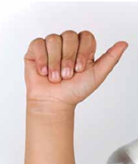
\includegraphics[width=4cm]{Images/Cap 2/Alfabeto LSM/A.png}}} \\
    \hline
    
    B & Los dedos índice, medio, anular y meñique se estiran unidos, y el pulgar se dobla hacia la palma, la cual mira al frente.
    & \makecell{\colorbox{white}{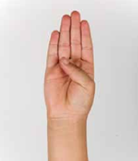
\includegraphics[width=4cm]{Images/Cap 2/Alfabeto LSM/B.png}}} \\
    \hline
    
    C & Los dedos índice, medio, anular y meñique se mantienen unidos y en posición cóncava; el pulgar también se coloca en esa posición. La palma mira a un lado.
    & \makecell{\colorbox{white}{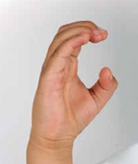
\includegraphics[width=4cm]{Images/Cap 2/Alfabeto LSM/C.png}}} \\
    \hline

    D & Los dedos medio, anular, meñique y pulgar se unen por las puntas y el dedo índice se estira. La palma mira al frente.
    & \makecell{\colorbox{white}{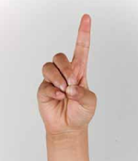
\includegraphics[width=4cm]{Images/Cap 2/Alfabeto LSM/D.png}}} \\
    \hline

    E & Se doblan los dedos completamente y se muestran las uñas. La palma mira al frente.
    & \makecell{\colorbox{white}{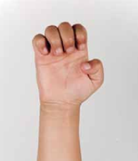
\includegraphics[width=4cm]{Images/Cap 2/Alfabeto LSM/E.png}}} \\
    \hline

    F & Con la mano abierta y los dedos unidos, se dobla el índice hasta que su parte lateral toque la yema del pulgar. La palma mira a un lado.
    & \makecell{\colorbox{white}{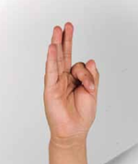
\includegraphics[width=4cm]{Images/Cap 2/Alfabeto LSM/F.png}}} \\
    \hline

    G & Se cierra la mano y los dedos índice y pulgar se estiran. La palma mira hacia la persona que se comunica.
    & \makecell{\colorbox{white}{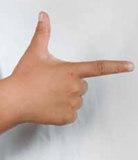
\includegraphics[width=4cm]{Images/Cap 2/Alfabeto LSM/G.png}}} \\
    \hline

    H & Se cierra la mano y los dedos índice y medio se unen y se estiran, se extiende el dedo pulgar señalando hacia arriba. La palma mira hacia la persona que se comunica.
    & \makecell{\colorbox{white}{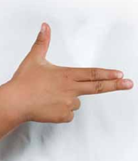
\includegraphics[width=4cm]{Images/Cap 2/Alfabeto LSM/H.png}}} \\
    \hline

    I & Con la mano cerrada, el dedo meñique se estira señalando hacia arriba. La palma se coloca de lado.
    & \makecell{\colorbox{white}{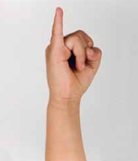
\includegraphics[width=4cm]{Images/Cap 2/Alfabeto LSM/I.png}}} \\
    \hline

    J & Con la mano cerrada, el dedo meñique estirado señala hacia arriba y la palma señala a un lado. La mano dibuja una “j” en el aire.
    & \makecell{\colorbox{white}{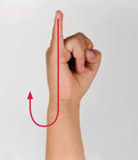
\includegraphics[width=4cm]{Images/Cap 2/Alfabeto LSM/J.png}}} \\
    \hline

    K & Se cierra la mano con los dedos índice, medio y pulgar estirados. La yema del pulgar se coloca entre el índice y el medio, moviendo la muñeca hacia arriba.
    & \makecell{\colorbox{white}{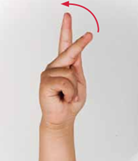
\includegraphics[width=4cm]{Images/Cap 2/Alfabeto LSM/K.png}}} \\
    \hline

    L & Con la mano cerrada y los dedos índice y pulgar estiados, se forma una “L”. La palma mira al frente.
    & \makecell{\colorbox{white}{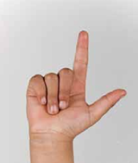
\includegraphics[width=4cm]{Images/Cap 2/Alfabeto LSM/L.png}}} \\
    \hline

    M & Con la mano cerrada, se ponen los dedos índice, medio y anular sobre el pulgar.
    & \makecell{\colorbox{white}{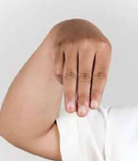
\includegraphics[width=4cm]{Images/Cap 2/Alfabeto LSM/M.png}}} \\
    \hline
 
    N & Con la mano cerrada, se ponen los dedos índice y medio sobre el pulgar. 
    & \makecell{\colorbox{white}{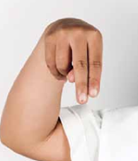
\includegraphics[width=4cm]{Images/Cap 2/Alfabeto LSM/N.png}}} \\
    \hline

    Ñ & Con la mano cerrada, se ponen los dedos índice y medio sobre el pulgar. Se mueve la muñeca a los lados. 
    & \makecell{\colorbox{white}{\includegraphics[width=4cm]{Images/Cap 2/Alfabeto LSM/Ñ.png}}} \\
    \hline

    O & Con la mano se forma una letra “o”. Todos los dedos se tocan por las puntas. 
    & \makecell{\colorbox{white}{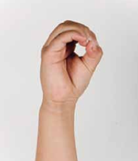
\includegraphics[width=4cm]{Images/Cap 2/Alfabeto LSM/O.png}}} \\
    \hline

    P & Con la mano cerrada y los dedos índice, medio y pulgar estirados, se coloca la yema del pulgar entre el índice y el medio.
    & \makecell{\colorbox{white}{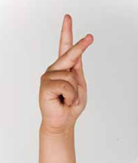
\includegraphics[width=4cm]{Images/Cap 2/Alfabeto LSM/P.png}}} \\
    \hline
    
    Q & Con la mano cerrada, se colocan los dedos índice y pulgar en posición de garra. La palma mira hacia abajo, y se mueve hacia los lados.
    & \makecell{\colorbox{white}{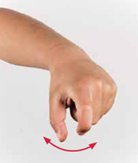
\includegraphics[width=4cm]{Images/Cap 2/Alfabeto LSM/Q.png}}} \\
    \hline
    
    R & Con la mano cerrada, se estiran y entrelazan los dedos índice y medio. La palma mira al frente.
    & \makecell{\colorbox{white}{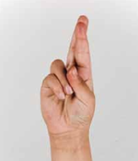
\includegraphics[width=4cm]{Images/Cap 2/Alfabeto LSM/R.png}}} \\
    \hline

    S & Con la mano cerrada, se pone el pulgar sobre los otros dedos. La palma mira al frente.
    & \makecell{\colorbox{white}{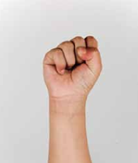
\includegraphics[width=4cm]{Images/Cap 2/Alfabeto LSM/S.png}}} \\
    \hline

    T & Con la mano cerrada, el pulgar se pone entre el índice y el medio. La palma mira al frente. 
    & \makecell{\colorbox{white}{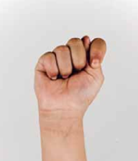
\includegraphics[width=4cm]{Images/Cap 2/Alfabeto LSM/T.png}}} \\
    \hline

    U & Con la mano cerrada, se estiran los dedos índice y medio unidos. La palma mira al frente. 
    & \makecell{\colorbox{white}{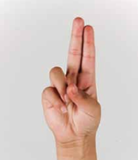
\includegraphics[width=4cm]{Images/Cap 2/Alfabeto LSM/U.png}}} \\
    \hline

    V & Con la mano cerrada, se estiran los dedos índice y medio separados. La palma mira al frente. 
    & \makecell{\colorbox{white}{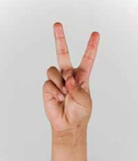
\includegraphics[width=4cm]{Images/Cap 2/Alfabeto LSM/V.png}}} \\
    \hline

    W & Con la mano cerrada, se estiran los dedos índice, medio y anular separados. La palma mira al frente. 
    & \makecell{\colorbox{white}{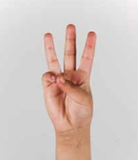
\includegraphics[width=4cm]{Images/Cap 2/Alfabeto LSM/W.png}}} \\
    \hline

    X & Con la mano cerrada, el índice y el pulgar en posición de garra y la palma dirigida a un lado, se realiza un movimiento al frente y de regreso. 
    & \makecell{\colorbox{white}{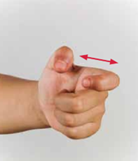
\includegraphics[width=4cm]{Images/Cap 2/Alfabeto LSM/X.png}}} \\
    \hline
    
    Y & Con la mano cerrada, se estira el meñique y el pulgar. La palma mira hacia la persona que se comunica. 
    & \makecell{\colorbox{white}{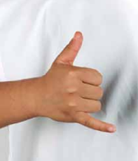
\includegraphics[width=4cm]{Images/Cap 2/Alfabeto LSM/Y.png}}} \\
    \hline

    Z & Con la mano cerrada, el dedo índice estirado y la palma al frente, se dibuja una letra z en el aire. 
    & \makecell{\colorbox{white}{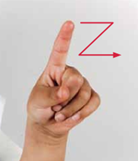
\includegraphics[width=4cm]{Images/Cap 2/Alfabeto LSM/Z.png}}} \\
    \hline
    
    \caption{Abecedario LSM, obtenido de [s91].} \label{tabla:LSM}
\end{longtable}
    
\newpage
\subsection{Dactilogía}
La dactilología es un sistema de comunicación que transmite información mediante el deletreo manual, y en ocasiones es usado en conjunto con la lengua de señas. Se emplea la mano de diferente manera para pronunciar cada una de las letras [s22].\\

Otra definición de la dactilología es que es la representación manual de cada una de las letras que componen el alfabeto, para poder transmitir a las personas sordas cualquier palabra que se desee comunicar. Todas las lenguas de señas poseen mecanismos internos que les permiten generar mensajes [s23].\\

Para comunicarse por medio de dactilología se emplea la mano dominante a la altura de la barbilla, en conjunto con la articulación oral, siendo necesario que la cara y la boca sean visibles [s23]. Principalmente se usa para sustantivos, nombres propios, direcciones y palabras para los cuales no existe un signo creado.\\

Si bien la discapacidad auditiva representa una barrera de la comunicación, las personas sordas en los últimos años han buscado superar esa barrera con ayuda de dispositivos tecnológicos que puedan fungir como intérpretes. El desarrollo de la Inteligencia Artificial (IA), más concretamente las técnicas de Procesamiento de Lenguaje Natural (PLN) y modelado de animaciones 3D, han ayudado a crear nuevos sistemas que faciliten la interacción entre personas oyentes y personas de la comunidad sorda, derribando las barreras de la comunicación. 

\section{Inteligencia Artificial}
La Inteligencia Artificial (IA) es la capacidad que poseen las máquinas para usar algoritmos y aprender de los datos para tomar decisiones tal como lo haría un ser humano [s3]. A diferencia del ser humano, la IA no necesita descansar y es capaz de analizar grandes cantidades de información, reduciendo el margen de error.\\

La IA se basa en el uso de algoritmos y tecnologías de aprendizaje automático para dar a las máquinas la capacidad de aplicar ciertas habilidades cognitivas y realizar tareas por sí mismas de manera autónoma o semiautónoma. A medida que la IA mejora, muchos procesos son más eficientes y algunas tareas que parecían complicadas se realizan con mayor rapidez y precisión [s31].\\

\subsection{Clasificación de la Inteligencia Artificial}
La IA puede ser clasificada de varias maneras, ya sea a partir de su grado de capacidad cognitiva o a partir de su grado de autonomía [s31].\\

\textbf{Clasificación a partir de su grado de capacidad cognitiva:}
\begin{itemize}
    \item Inteligencia Artificial débil o limitada. Está diseñada para realizar tareas específicas de manera eficiente, pero no tiene la capacidad de razonar ni aprender de nuevas situaciones [s31].\\
\item Inteligencia Artificial general o fuerte. Este tipo de IA tiene la capacidad de realizar varias tareas cognitivas como el razonamiento, el aprendizaje y la resolución de problemas. A diferencia de la IA débil, la IA fuerte es capaz de adaptarse a nuevas situaciones y entornos [s31].\\
\item Super Inteligencia Artificial. Tiene la capacidad de realizar cualquier tarea compleja que requiere Inteligencia Humana, ya que es muy poderosa, y puede superar a los seres humanos en términos de capacidad cognitiva y de aprendizaje [s31].\\

\end{itemize}

\textbf{Clasificación de acuerdo con su grado de autonomía:}

\begin{itemize}
    \item Inteligencia Artificial Reactiva. Este tipo de IA realiza tareas específicas de manera autónoma, pero no tiene la capacidad de recordar eventos pasados ni de anticipar situaciones futuras. Es útil en situaciones en las que se requieren respuestas rápidas y precisas a situaciones específicas [s31].\\
\item Inteligencia Artificial Deliberativa. Tiene la capacidad de planificar y tomar decisiones basándose en información del entorno y en objetivos predeterminados. Es decir, puede analizar situaciones y elegir opciones que le permitan cumplir con objetivos, o adaptarse a entornos empleando información del pasado y del futuro [s31].\\

\item Inteligencia Artificial Cognitiva. Se caracteriza por su capacidad de imitar las funciones cognitivas humanas como lo son el razonamiento, la percepción y el aprendizaje, y tienen la capacidad de adaptarse a nuevas situaciones y entornos [s31].\\

\item Inteligencia Artificial Autónoma. Es capaz de interactuar de manera autónoma con su entorno, tomar decisiones y aprender de nuevas situaciones, y cambiar sus objetivos y estrategias en función de las estrategias sin la necesidad de la intervención humana [s31].

\end{itemize}

De igual manera, la IA emplea diferentes técnicas, las cuales se enlistan a continuación [s4]:

\begin{itemize}
    \item Búsqueda de soluciones. Tiene por objetivo encontrar mecanismos de deducción y búsqueda de soluciones para la resolución de problemas cuando no se cuenta con un método directo [s4].\\
\item Representación del conocimiento. Elaboración de métodos y técnicas eficientes que sean capaces de organizar conocimientos en un sistema, para posteriormente ser usados en la búsqueda de soluciones para diferentes problemáticas [s4].\\
\item Reconocimiento de patrones. Son técnicas de clasificación para identificar subgrupos midiendo el parecido o similitud entre formas, con el objetivo de obtener conclusiones [s4].\\
\item Robótica. Esta técnica tiene por objetivo la construcción de robots inteligentes capaces de funcionar con autonomía, que cuenten con la habilidad de realizar procesos mecánicos y manuales con el fin de obtener mayor productividad, suplir mano de obra y proporcionalidad flexibilidad en procesos industriales [s4].\\
\item Redes Neuronales. Son sistemas compuestos por estructuras de red, con un gran número de conexiones entre diferentes capas de procesadores, que a su vez tienen asignadas diferentes funciones. Las redes neuronales efectúan una labor de aprendizaje por la reproducción de las salidas de un conjunto de entrenamiento [s4].\\
\item Algoritmos genéticos. Son los tipos de algoritmos que tratan de emular el proceso de selección natural a un problema dado, en el que se aplican operadores genéticos para evaluar cada una de las soluciones propuestas. Se emplean procedimientos de búsqueda y optimización para mejorar las soluciones existentes y generar nuevas [s4].\\
\item Sistemas expertos. Sistemas que almacenan conocimientos de expertos sobre un área o campo especializado, para obtener una solución mediante una deducción lógica [s4]. \\
\item Procesamiento de Lenguaje Natural (PLN). El PLN se centra en el diseño de métodos y algoritmos que toman como entrada o producen como salida datos en la forma del lenguaje humano, ya sea en forma de texto, audio o animación [s41].

\end{itemize}

En este Trabajo Terminal nos centraremos en la técnica de Procesamiento de Lenguaje Natural (PLN). En el siguiente apartado se profundizará más en el concepto, características y usos del PLN.\\

\section{Procesamiento de Lenguaje Natural (PLN)}
El Procesamiento de Lenguaje Natural (PLN, o NLP por sus siglas en inglés) es el campo de estudio que busca entender cómo funciona el lenguaje, su construcción, la generación de nuevo lenguaje, así como todas las tareas que tienen relación con el tratamiento del lenguaje como lo es la generación de texto, traductores, generadores de resúmenes, chatbots, entre otros [s44].\\

El PLN emplea el lenguaje natural para establecer comunicación entre un ser humano y una computadora. Esta última deberá entender las oraciones que le sean proporcionadas mediante modelos que le ayuden a entender los mecanismos humanos relacionados con el lenguaje [s43]. 


\subsection{Arquitectura de un sistema de PLN}

La arquitectura de un sistema de PLN está dividida en niveles:\

\begin{enumerate}[label=\alph*.]
    \item \textbf{Nivel Fonológico.} Explica cómo es que las palabras se relacionan con los sonidos que representan.
    \item \textbf{Nivel Morfológico.} Indica cómo es que las palabras se construyen a partir de unidades de significado más pequeñas llamadas morfemas.
    \item \textbf{Nivel Sintáctico.} Se analiza cómo es que las palabras se unen para formar oraciones, entendiendo la función estructural que cada palabra posee.
    \item \textbf{Nivel Semántico.} Se refiere al significado de las palabras, y cómo los mismos se unen para darle sentido a una oración, considerando también el contexto de la oración.
    \item \textbf{Nivel Pragmático.} Trata de cómo las oraciones son empleadas en diferentes situaciones y cómo es que el uso afecta el significado de las mismas.
\end{enumerate}

\begin{center}
    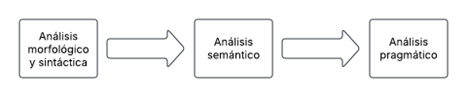
\includegraphics[width=0.8\textwidth]{Images/diagraanali.png}
    \captionof{figure}{Arquitectura de un Sistema de Procesamiento de Lenguaje Natural, obtenido de [s43].}  % Pie de foto manual
\end{center}

\textbf{Los pasos que sigue la arquitectura del sistema de PLN es la siguiente [s43]:}
\begin{enumerate}
    \item El usuario le expresa a la computadora lo que desea hacer.\\
    \item La computadora analiza las oraciones que el usuario le proporciona, en el sentido morfológico y sintáctico. Es decir, se verifican los componentes léxicos definidos y se verifica si se cumple un orden gramatical entre los elementos identificados.\\
    \item Posteriormente, se realiza un análisis sintáctico de las oraciones, para saber cuál es el significado de cada oración.\\
    \item Después de realizar el paso anterior, se lleva a cabo un análisis pragmático de todas las oraciones juntas. Al final de este paso, la computadora obtiene la expresión final.\\
    \item Una vez obtenida la expresión final, la misma es ejecutada para obtener un resultado que será proporcionado al usuario.
\end{enumerate}

\subsection{Técnicas de PLN}
El PLN se apoya de un conjunto de técnicas mediante las cuales se extrae información determinada de un texto. A continuación, se describen algunas de las técnicas más comunes utilizadas:

\begin{enumerate}
    \item Detección de oraciones. La detección de oraciones es una de las técnicas básicas correspondientes al  nivel de procesamiento sintáctico, que funciona recortando una secuencia de caracteres entre dos signos de puntuación; el signo debe estar acompañado por un espacio en blanco y se excluye el caso de la primer frase, y en posibles ocasiones la última frase.\\
    
La detección de oraciones puede presentar algunas dificultades a la hora de procesar títulos, abreviaturas, o algunos elementos que no siguen algún patrón de texto plano. En el caso de las abreviaturas, se utilizan palabras cargadas en el modelo, empleando un modelo por idioma, ya que el mismo posee los símbolos o abreviaturas necesarias para detectar las sentencias [s46].
\begin{center}
    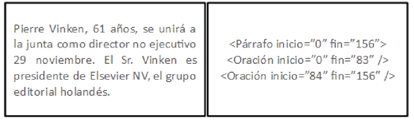
\includegraphics[width=0.8\textwidth]{Images/lib.png}
    \captionof{figure}{Ejemplo de la delimitación de oraciones dentro de un párrafo, obtenido de [s46].}  % Pie de foto manual
\end{center}
El ejemplo anterior muestra que el modelo en español determina que “Sr.” es una abreviatura de la palabra “Señor”, y por consiguiente ignora el signo de puntuación como final de la oración.

\item Segmentación por palabras. Después de que se identificaron cada una de las oraciones que componen el texto, se procede a la segmentación por palabras, más conocida como analizador léxico o “Tokenizer”. 
Esta técnica pertenece al nivel léxico y consiste en la identificación de tokens, que son unidades lingüísticas como palabras, puntuación, números, caracteres alfanuméricos, etc. Para identificar tokens en idiomas modernos, se delimitan espacios en blanco con límites de palabra, entre comillas, paréntesis y puntuación.
El trato con las abreviaciones es similar a la detección de oraciones, ya que no existen normas universalmente aceptadas para muchas abreviaturas y acrónimos. En el caso del reconocimiento de abreviaturas, se mantiene una lista de palabras recortadas reconocidas [s46].
\begin{center}
    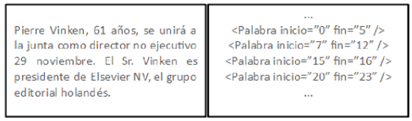
\includegraphics[width=0.8\textwidth]{Images/lib2.png}
    \captionof{figure}{ Ejemplo de separación de palabras en un párrafo, obtenido de [s46].}  % Pie de foto manual
\end{center}
En el ejemplo anterior, se obtiene la lista de palabras del texto, con la separación por palabras indicada por los espacios en blanco y los signos de puntuación. 

\item Etiquetado gramatical o Part-of-Speech (POS) - tagging. Posterior a la ejecución de las dos técnicas previamente explicadas, se puede realizar el proceso de etiquetado de palabras de acuerdo con el rol que cumplen dentro de una oración. El proceso de Etiquetado gramatical consiste en asignar a cada una de las palabras de un texto su categoría gramatical de acuerdo con la definición de la misma o el contexto en el que aparece, como lo pueden ser los sustantivos, adjetivos, adverbios, etc.

Para lograr lo anterior, se necesita establecer las relaciones de una palabra con sus adyacentes dentro de una frase o de un párrafo. Un mismo token puede tener múltiples etiquetas POS, pero solo una es válida dependiendo del contexto.
\begin{center}
    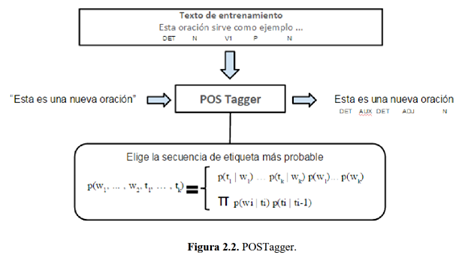
\includegraphics[width=0.8\textwidth]{Images/sec.png}
    \captionof{figure}{POS Tagger, obtenido de [s46].}  % Pie de foto manual
\end{center}
\item Segmentación morfológica. Un morfema se define como un fragmento mínimo capaz de expresar el significado de una palabra, es decir, es la unidad significativa más pequeña de un idioma.\\

Los morfemas se clasifican en 2 categorías. Los morfemas independientes admiten cierta libertad fonológica del lexema: 
\begin{itemize}
    \item Pronombres: cuíde-se, di-le, él, ella.
\item Preposiciones: desde, a, con, de.
\item Conjunciones: y, e, o, pero, aunque.
\item Determinantes: él, ella, ese, un, una.
\end{itemize}
Por otro lado, los morfemas dependientes van unidos a otra unidad mínima dotada de significado, conocidos como monemas, para completar su significado.  Los tipos de morfemas dependientes son: 

\begin{enumerate}
    \item Derivativos: estos morfemas son facultativos, es decir, añaden matices al significado de los lexemas.
    \begin{itemize}
        \item Prefijos
        \item Sufijos
        \item Interfijos
    \end{itemize}
    \item Flexivos: estos morfemas son constitutivos, es decir, señalan relaciones gramaticales y sus accidentes entre los diferentes agentes de una acción verbal o una expresión nominal.
    \begin{itemize}
        \item Género
\item Número
\item Persona
\item Modo y tiempo
    \end{itemize}

\end{enumerate}
La identificación de monemas permite el análisis en profundidad de una palabra en un texto, ya que de esta forma se obtiene información específica como el género, modo, tiempo, etc. y es posible ubicar de manera precisa cada palabra de una oración.

\item Eliminación de Stop Words. Mediante esta técnica, se excluyen palabras comunes que tienen poco valor para la recuperación de información. La cantidad de ocurrencias de una palabra en un texto determina si es o no una “stop word”, siendo que cuanto más ocurrencias existan menos relevancia tiene en el texto; en su mayoría, los artículos, los pronombres, las preposiciones y las conjunciones. La técnica de eliminación de stop words permite reducir el tamaño de un texto, eliminando aproximadamente el 30\% o 40\% de las palabras, y se seleccionan las palabras claves. \\

A partir de un listado de palabras Stop words, se detectan dentro del texto para su posible eliminación. En ocasiones, al listado de palabras de uso común se le agrega un conjunto de palabras propias del documento que se analiza, empleando la técnica TF-IDF (Term Frequency - Inverse Document Frequency), que permite determinar qué palabras son importantes para un documento de acuerdo con la frecuencia de aparición dentro de un texto.
\begin{center}
    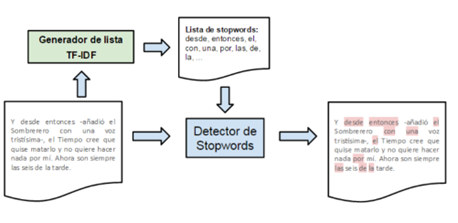
\includegraphics[width=0.8\textwidth]{Images/stop.png}
    \captionof{figure}{ Ejemplo de Detección de Stop words, obtenido de [s34].}  % Pie de foto manual
\end{center}

\item Reconocimiento de Entidades Nombradas (NER). Busca y clasifica elementos de texto que pertenecen a categorías predefinidas, como lo son nombres de personas, entidades, organizaciones, lugares, expresiones temporales, cantidades, porcentajes. etc.
Para poder hacer el reconocimiento de las diferentes entidades, se utilizan una serie de aproximaciones, y para poder realizar el análisis es necesario tener una noción del contexto en el cual se encuentra cada una de las entidades para determinar a qué se refieren. Finalmente, dentro de las posibles entidades se realiza una asociación con los conceptos del contexto dentro de una base de datos de conocimiento.
\begin{center}
    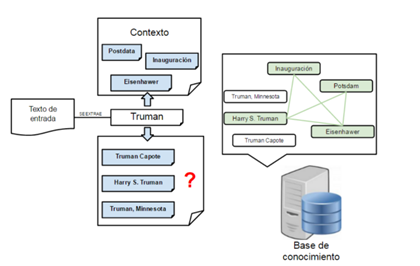
\includegraphics[width=0.8\textwidth]{Images/truman.png}
    \captionof{figure}{Reconocimiento de Entidades Nombradas, obtenido de [s46]
}  % Pie de foto manual
\end{center}
\item Stemming. Esta técnica busca un concepto de una palabra mediante la eliminación de prefijos y sufijos para obtener la raíz. De esta manera, se reduce la palabra a su mínimo elemento con significado

\begin{center}
    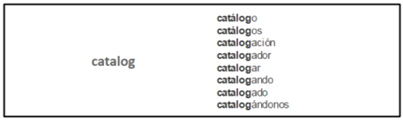
\includegraphics[width=0.8\textwidth]{Images/catalog.png}
    \captionof{figure}{Ejemplo de los términos derivados de la raíz “catalog”, obtenido de [s46].}  % Pie de foto manual
\end{center}
No obstante, es importante mencionar que esta técnica no siempre funciona correctamente debido a que hay palabras que poseen raíces compartidas por más de un significado. 
\begin{table}[h]
    \centering
    \begin{tabular}{|p{4cm}|p{3cm}|p{5cm}|}
        \hline
        \textbf{Término con prefijo} & \textbf{Raíz/Stem} & \textbf{Término con el que causaría confusión} \\
        \hline
        Prevalencia & valenc & Valencia, valencia, valenciano, ambivalencia, polivalencia \\
        \hline
        Precatalogar & catalog & Descatalogar, catálogo \\
        \hline
    \end{tabular}
    \caption{Ejemplos de términos con raíces compartidas, obtenido de [s46]}
    \label{tabla:confusion}
\end{table}

\end{enumerate}

\subsection{Aplicaciones del PLN}
A continuación, se enlistan las principales aplicaciones del PLN:
\begin{itemize}
    \item Recuperación y extracción de información. La recuperación de información (RI), es el proceso de encontrar en un repositorio grande de datos, material (usualmente documentos) de naturaleza no estructurada (usualmente texto) o semiestructurada (páginas Web, por ejemplo), que satisfaga una necesidad de información [s45].
    \item Por su parte, la extracción de información (EI) consiste en la obtención de las partes de las partes que interesan en el texto para pasarlas a un formato de base de datos [s45].
    \item Minería de datos. La minería de datos proporciona herramientas poderosas para descubrir patrones ocultos y relaciones en datos estructurados. Este proceso asume que los datos ya se encuentran almacenados en un formato estructurado. La minería de datos usa técnicas y metodologías de reconocimiento de información, extracción de información y corpus procesados con técnicas de lingüística computacional [s45].
    \item Sistemas de búsqueda de respuestas. Son sistemas diseñados para tomar una pregunta en lenguaje natural y proporcionar una respuesta, para evitar que los usuarios naveguen y lean varias páginas de resultados de búsqueda. Estos sistemas son construidos sobre motores de búsqueda y requieren contenido fuente para descubrir las respuesta; a su vez, deben tener métodos para entender las preguntas del usuario y determinar el tipo de respuesta que debe dar [s45].
    \item Generación de resúmenes automáticos. La generación de resúmenes consiste en emplear herramientas de PLN, dichos resúmenes pueden ser con enfoque extractivo o abstractivo. Por un lado, los métodos extractivos consisten en tomar una colección de términos, frases o párrafos significativos que definen el significado del texto original para generar un resumen. Por otro lado, los métodos abstractivos dependen de técnicas de parafraseo para producir las síntesis, las técnicas aún están siendo desarrolladas [s45].
    \item Análisis de sentimientos. El análisis de sentimientos en textos es la identificación y extracción de información subjetiva. Este proceso generalmente involucra el uso de herramientas de PLN y software de análisis de textos para automatizar el proceso. La forma básica de análisis de sentimientos es una clasificación polarizada de sentimientos que puede asignar calificaciones de en un rango de -10 a 10 que se basa en el aprendizaje para evaluar emociones tanto negativas como positivas en corpus etiquetados de entrenamiento [s45].
    \item Traducción automática. Consiste en tomar el texto escrito en un lenguaje y traducirlo a otro, manteniendo el mismo significado. El proceso de traducción automática sigue tres pasos: en primer lugar, el texto en el lenguaje original se transforma a una representación intermedia, luego se realizan modificaciones a esta representación intermedia basándose en la morfología del lenguaje, y finalmente se transforma al lenguaje destino [s45].

\end{itemize}

\section{MediaPipe}
MediaPipe es un conjunto de herramientas de código abierto para ser empleadas en tareas como el reconocimiento facial, seguimiento de gestos, detección de objetos y el seguimiento del cuerpo humano [s5].
\subsection{Herramientas de MediaPipe}
Las principales herramientas que ofrece MediaPipe son:
\begin{itemize}
    \item MediaPipe Detección de caras. Permite detectar y seguir rostros de una imagen o vídeos en tiempo real, empleando técnicas de machine learning para mejorar la precisión [s5].
    \item Malla facial MediaPipe. Proporciona una malla 3D del rostro, para proporcionar información precisa sobre los rasgos faciales, lo cuál es útil en aplicaciones de animación y modelado 3D [s5].
    \item MediaPipe Seguimiento manual. Con esta herramienta se puede detectar y seguir los movimientos de la mano en tiempo real, con alta precisión [s5].
    \item MediaPipe Holistic. Combina la detección facial, el seguimiento de manos y el seguimiento corporal en una sola herramienta integrada, lo que es útil para aplicaciones de realidad aumentada y juegos [s5].
    \item MediaPipe Objectron. Es una herramienta para detectar y seguir objetos 3D en el espacio, siendo útil para comprender e interactuar con objetos reales en un entorno virtual [s5].
    \item Segmentación MediaPipe Selfie. Permite segmentar a las personas en el fondo de una imagen o vídeo [s5].
    \item MediaPipe Pose. Detecta las posturas del cuerpo humano, proporcionando información sobre las posiciones de las articulaciones y las extremidades [s5].
    \item Reconocimiento de gestos MediaPipe. Herramienta empleada en el reconocimiento de gestos de la mano para interacciones intuitivas y control de gestos [s5].
    \item MediaPipe EfficientDet. Mediante el uso de Redes Neuronales rápidas y eficaces, se puede mejorar la detección y localización de objetos en imágenes [s5]. 

\end{itemize}
\subsection{MediaPipe Pose}
Como se comentó en el apartado anterior, MediaPipe Pose permite detectar puntos de referencia de cuerpos humanos en una imagen o vídeo. Se emplea principalmente para identificar ubicaciones claves del cuerpo, analizar la postura y categorizar los movimientos [s51].

El marcador de poses emplea una serie de modelos para predecir los marcadores de poses [s51]:
\begin{itemize}

    \item Modelo de detección de poses. Detectar la presencia de cuerpos con algunos puntos de referencia de poses clave.
    \item Modelo de marcador de pose. Agregar una asignación completa de una pose, en la que se generan 33 puntos de referencia de la pose 3D.

\end{itemize}
El modelo de marcador de pose realiza un seguimiento de 33 ubicaciones de puntos de referencia del cuerpo.
\begin{center}
    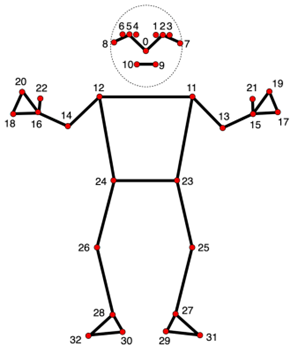
\includegraphics[width=0.8\textwidth]{Images/human.png}
    \captionof{figure}{Ubicaciones de puntos de referencia del cuerpo [s51].}  % Pie de foto manual
\end{center}
A continuación, se enlistan las partes representadas del cuerpo:

\begin{enumerate}
    \item Nose - nariz  
    \item Left eye (inner) - ojo izquierdo (interior)  
    \item Left eye - ojo izquierdo  
    \item Left eye (outer) - ojo izquierdo (exterior)  
    \item Right eye (inner) - ojo derecho (interior)  
    \item Right eye - ojo derecho  
    \item Right eye (outer) - ojo derecho (exterior)  
    \item Left ear - oreja izquierda  
    \item Right ear - oreja derecha  
    \item Mouth (left) - boca (izquierda)  
    \item Mouth (right) - boca (derecha)  
    \item Left shoulder - hombro izquierdo  
    \item Right shoulder - hombro derecho  
    \item Left elbow - codo izquierdo  
    \item Right elbow - codo derecho  
    \item Left wrist - muñeca izquierda  
    \item Right wrist - muñeca derecha  
    \item Left pinky - meñique izquierdo  
    \item Right pinky - meñique derecho  
    \item Left index - índice izquierdo  
    \item Right index - índice derecho  
    \item Left thumb - pulgar izquierdo  
    \item Right thumb - pulgar derecho  
    \item Left hip - cadera izquierda  
    \item Right hip - cadera derecha  
    \item Left knee - rodilla izquierda  
    \item Right knee - rodilla derecha  
    \item Left ankle - tobillo izquierdo  
    \item Right ankle - tobillo derecho  
    \item Left heel - talón izquierdo  
    \item Right heel - talón derecho  
    \item Left foot index - punta del pie izquierdo  
    \item Right foot index - punta del pie derecho  
\end{enumerate}

\section{Modelado de Animaciones 3D}
El término animación 3D se refiere a la técnica de animación empleada para desplazar modelos tridimensionales generados digitalmente, sirviéndose para ello de un eje de coordenadas cartesiano virtual [s7].\\

La animación 3D ha estado históricamente más orientada a la replicación de la física del mundo real, ya que representa con total libertad la fuerza de gravedad, la inercia o la masa de cuerpos [s7].

\subsection{Unity}
Unity es una plataforma para el desarrollo de videojuegos y aplicaciones interactivas, que ofrece una amplia variedad de herramientas y recursos para crear experiencias visuales y funcionales [s8]. Es un motor gráfico empleado para desarrollar videojuegos, aplicaciones interactivas en 2D, 2D, realidad aumentada (AR) y realidad virtual (VR), y tiene soporte en varias plataformas como PC, consolas, dispositivos móviles y dispositivos de realidad extendida [s8].\\

Unity destaca por su conjunto de características robustas que facilitan el desarrollo de aplicaciones interactivas de alta calidad para la simulación física y el rendering, las cuáles requieren visualización y experiencia de usuario de alta calidad [s8].\\

En la actualidad Unity es empleado en múltiples industrias, además del desarrollo de videojuegos, ya que es popular en sectores como la arquitectura, el diseño automotriz, la medicina y la educación. 



\section{Sistema Operativo Android}
Un sistema operativo móvil es un conjunto de programas que habilitan características específicas de un teléfono móvil y brindan servicios a las aplicaciones móviles que se ejecutan en él [s81].\\

El sistema operativo Android es un sistema operativo móvil desarrollado por la empresa estadounidense Google y que está basado en el sistema operativo Linux. Es un sistema operativo abierto, gratuito, versátil, seguro y altamente personalizable que está desarrollado para dispositivos móviles como smartphones y tablets [s81].

Las principales características de Android son las siguientes [s81]:

\begin{itemize}

    \item Interfaz de Usuario (UI) personalizable. Los usuarios son capaces de cambiar el aspecto de sus dispositivos para adaptarlos a sus necesidades.
    \item Compatibilidad con múltiples fabricantes. Este sistema operativo es ejecutado en una gran cantidad de dispositivos de múltiples fabricantes.
    \item Google Play Store. Android cuenta con una tienda de aplicaciones que permite descargar diferentes aplicaciones de diversa índole, basadas en las necesidades de cada usuario.
    \item Asistente Virtual. Los usuarios tienen acceso a un asistente virtual llamado Google Assistant, que ayuda en la realización de tareas.
    \item Integración con servicios de Google. Android está integrado con servicios de Google como Gmail, Google Drive, Google Photos, Maps, entre otros.
    \item Compatibilidad con tecnologías emergentes. Android es compatible con tecnologías como la Realidad Virtual (VR), la Realidad Aumentada (AR) y los asistentes virtuales. 
\end{itemize}
